% Pokec-z — Fairness multi-axes par composition d'outils post-hoc
% Source LaTeX du 2-pager. Compilable avec pdflatex (TeX Live ou MiKTeX).
% Les figures sont dans le même répertoire (fig1_*.png, fig2_*.png).
%
% Compilation :
%   pdflatex 2_pager.tex
%
% Note : la version de référence est 2_pager.md (rendu via scripts/build_pdf.py
% en utilisant la lib Python markdown-pdf). Ce fichier .tex est une
% transcription manuelle pour permettre la compilation pdflatex en plus.

\documentclass[10pt,a4paper]{article}

\usepackage[T1]{fontenc}
\usepackage[utf8]{inputenc}
\usepackage[french]{babel}
\usepackage{lmodern}
\usepackage[a4paper,margin=1.0cm,top=1.0cm,bottom=1.0cm]{geometry}
\usepackage{graphicx}
\usepackage{booktabs}
\usepackage{array}
\usepackage{multirow}
\usepackage{caption}
\usepackage{xcolor}
\usepackage{hyperref}
\usepackage{enumitem}
\usepackage{textcomp}

% Layout serré pour tenir 2 pages.
\setlength{\parindent}{0pt}
\setlength{\parskip}{0.25em}
\renewcommand{\baselinestretch}{1.05}
\setlist[itemize]{leftmargin=1.2em,topsep=0.1em,itemsep=0.05em}
\setlist[enumerate]{leftmargin=1.4em,topsep=0.1em,itemsep=0.05em}

% Caption italique gris, comme dans la version markdown.
\captionsetup{font={small,it},labelfont={bf},labelsep=period,
              textfont={color=gray!70!black}}

\hypersetup{colorlinks=true,linkcolor=black,urlcolor=blue!50!black}

\title{\vspace{-2.5em}Pokec-z — Fairness multi-axes par composition d'outils post-hoc}
\author{}
\date{}

\begin{document}
\maketitle\vspace{-3em}

\noindent\textbf{Mini-projet IADATA708.} Branche \texttt{feature/fairgnn-fix-and-multi-fairness}.

\section{Setup}

\textbf{Données.} Pokec-z (subset officiel FairGNN, \textit{Žilinský kraj}) :
66\,569 nœuds, $\sim$729\,k arêtes, 264 features tabulaires. Reproduction sur
\textbf{Pokec-n}. Cible : \texttt{completed\_level\_of\_education\_indicator}
(binaire, 47.7\,\% positif). Attributs sensibles : \texttt{gender},
\texttt{region} (binaires), \texttt{age\_group} (3 classes), plus les
intersections \texttt{gender}\,$\times$\,\texttt{age\_group} et
\texttt{gender}\,$\times$\,\texttt{region} — soit \textbf{5 axes} simultanés.

\textbf{Splits.} Stratifié $y \times \texttt{gender}$ 60/20/20. Multi-seed
\texttt{[3, 7, 21, 42, 99]}.

\textbf{Méthodes} (toolbox de 5 familles) :
\begin{itemize}
\item \textit{Baselines} : GraphSAGE (2 SAGE, hidden=256, dropout=0.5),
  \textbf{TabICL} (foundation tabulaire INRIA 2025, no graph, frozen).
\item \textit{Pre-process} : Resampling, FairDrop, Reweighting Kamiran-Calders 2012.
\item \textit{In-training} : \textbf{FairGNN avec Gradient Reversal Layer} —
  réimpl propre de Dai \& Wang 2021. La version originale combinait
  $l_{cls} - \lambda \cdot l_{adv}$ dans un seul optimiseur (pas du min-max),
  F1 collapsait à 0.4834 à certains $\lambda$.
\item \textit{Post-process} : EOT (Hardt 2016), DPT (Demographic Parity
  Threshold), \textbf{INLP} (Ravfogel 2020) sur embeddings et features, et
  \textbf{les compositions INLP+DPT et leur version multi-axes simultanée}.
\end{itemize}

\textbf{Métriques.} $\Delta$DP, $\Delta$EO, AUC gap (sortie),
\textbf{Sensitive Leakage AUC} (probe LR train$\to$test, Laclau et al.\ 2024).
50+ tests pytest, ruff propre, no-pandas/no-loops enforced.

\section{Finding 1 — Une toolbox, chaque outil sa métrique}

Notre résultat empirique principal sur cette première dimension est que
\textbf{les méthodes de fairness ne sont pas substituables}. Chaque famille
attaque une partie spécifique du problème, et il faut souvent en composer
plusieurs pour traiter les trois métriques en même temps.

\begin{figure}[h]
\centering
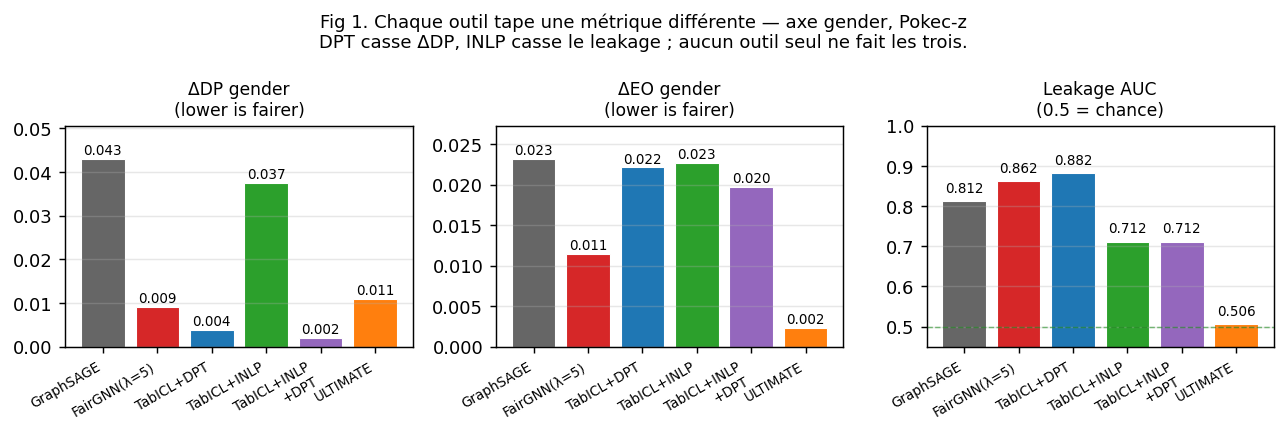
\includegraphics[width=0.95\linewidth]{fig1_toolbox_per_metric.png}
\caption*{\textit{Fig 1. Mêmes méthodes, 3 métriques. \textbf{DPT} (bleu)
écrase $\Delta$DP à 0.004 mais ne touche pas le leakage. \textbf{INLP}
(vert) tombe le leakage à 0.71 mais ne change pas $\Delta$DP. \textbf{FairGNN}
(rouge) bouge un peu les deux au prix de F1. Seul l'\textbf{ULTIMATE}
(orange = TabICL+INLP\_composite+DPT\_composite) règle les trois en même
temps.}}
\end{figure}

Pour un ingénieur qui voudrait une checklist, le mapping métrique $\to$ outil
est le suivant :

\begin{center}\small
\begin{tabular}{p{3.6cm} p{3.4cm} p{8.5cm}}
\toprule
\textbf{Si tu veux réduire\dots} & \textbf{Utilise} & \textbf{Pourquoi} \\
\midrule
\textbf{$\Delta$DP} (taux $\approx$ entre groupes) & \textbf{DPT} post-process & calibre un seuil par groupe, c'est l'objectif direct \\
\textbf{$\Delta$EO} (TPR $\approx$ entre groupes parmi $y=1$) & \textbf{EOT} post-process & même méca mais sur le sous-set $y=1$ \\
\textbf{Leakage} (sensible récupérable depuis embeddings) & \textbf{INLP} & projette l'espace orthogonal aux directions du sensible \\
\textbf{Tout en même temps} & \textbf{INLP\_composite + DPT\_composite} & les deux sont orthogonaux et se composent sans conflit \\
\bottomrule
\end{tabular}
\end{center}

Cette toolbox a une conséquence directe : \textbf{un foundation model + 30
lignes de post-process Pareto-domine FairGNN sur Pokec-z}. TabICL+EOT atteint
F1=0.946 et $\Delta$DP=0.007 contre FairGNN qui plafonne à F1=0.853 et
$\Delta$DP=0.009. On gagne 9 points de F1 \textit{et} on est légèrement plus
équitable, à un coût d'entraînement quasi-nul (TabICL est frozen, le
calibrage des seuils prend moins d'une seconde). C'est un résultat qui invite
à la prudence avant d'engager une méthode in-training adversariale
sophistiquée.

Le théorème de Chouldechova-Kleinberg (2017) dit par ailleurs que
$\Delta$DP=0 et $\Delta$EO=0 sont mathématiquement incompatibles dès que les
taux de base diffèrent entre groupes — ce qu'on vérifie expérimentalement :
DPT@\texttt{age\_group} baisse $\Delta$DP de 0.075 à 0.044 mais double
$\Delta$EO (0.034 $\to$ 0.074). Choisir une métrique n'est pas un choix
algorithmique, c'est un \textbf{choix normatif}.

\section{Finding 2 — TabICL tient la composition multi-axes, GraphSAGE s'écrase}

Le second résultat porte sur la \textbf{fairness sur plusieurs variables
simultanément} (\texttt{gender + age\_group + region}, encodés en attribut
composite à 12 cellules). Pour traiter cinq axes à la fois, il faut composer
INLP\_composite (latent) + DPT\_composite (sortie). C'est notre chaîne
ULTIMATE.

\begin{figure}[h]
\centering
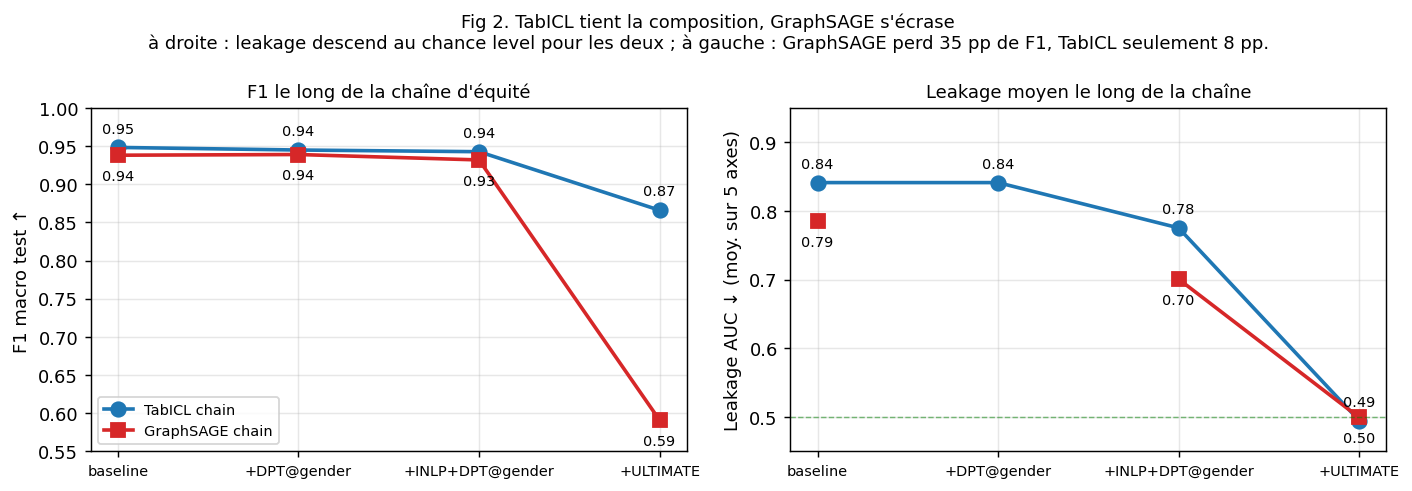
\includegraphics[width=0.95\linewidth]{fig2_chain_tabicl_vs_graphsage.png}
\caption*{\textit{Fig 2. F1 et leakage le long de la chaîne. À gauche :
TabICL garde F1=0.87 ; GraphSAGE chute à 0.59 (perte de 35 pp de F1). À droite :
les deux chaînes atteignent leakage = chance level (0.5).}}
\end{figure}

\textbf{Pourquoi GraphSAGE s'écrase et pas TabICL ?} Les coefficients
d'assortativité de Newman (2003) racontent toute l'histoire :
$r(\texttt{gender}) = -0.046$ (le graphe n'est pas du tout homophile en
gender), mais $r(\texttt{region}) = 0.901$ (le graphe est massivement
homophile en region). Le message passing de GraphSAGE recombine les features
d'un nœud avec celles de ses voisins ; quand ces voisins partagent presque
toujours la même region, l'embedding final encode la region beaucoup plus
intensément que la feature brute ne le laissait penser. Quand
INLP\_composite supprime ensuite les directions sensibles, il enlève une
part majeure de l'information utile et la représentation s'effondre. TabICL,
qui ne consomme jamais le graphe, n'a pas ce problème : ses embeddings ne
sont pas dominés par la region, donc INLP ne casse rien d'essentiel.

\textbf{La règle pratique qui en sort} est utilisable avant tout
entraînement : mesurer $r(s)$ pour chaque attribut sensible. Si $r(s)$ est
faible, le graphe n'aide pas à prédire la cible \textit{et} n'amplifie pas
le biais marginal, auquel cas un foundation model tabulaire + post-process
est presque toujours le bon choix. Si $r(s)$ est élevé (le cas typique des
datasets fairness-on-graphs publiés), les méthodes in-training graphiques
redeviennent nécessaires parce que le post-process, qui n'opère que sur les
sorties, ne peut pas atteindre l'espace latent biaisé. Sur Pokec-z,
$r(\texttt{gender}) = -0.046$ aurait dû nous orienter vers TabICL avant même
de lancer GraphSAGE.

La validation multi-seed \texttt{[3, 7, 21, 42, 99]} confirme la stabilité :
$\Delta$DP gender ULTIMATE = $0.006 \pm 0.005$ ; leakage gender =
$0.500 \pm 0.010$ ; F1 = 0.87 à dispersion marginale sur TabICL. La
reproduction sur Pokec-n donne les mêmes chiffres à un écart inférieur à 0.01.

\section{Compromis perf $\leftrightarrow$ équité $\leftrightarrow$ robustesse}

\textbf{Sur l'axe perf vs équité}, payer 8 points de F1 pour obtenir la
fairness multi-axes complète sur TabICL est un compromis défendable. Sur
GraphSAGE, perdre 35 points de F1 pour le même résultat de fairness rend la
chaîne inutilisable en production — c'est exactement le genre de situation
où le coût de la fairness fait basculer le choix d'architecture.

\textbf{Il n'y a pas de free-lunch intersectionnel.} Calibrer DPT uniquement
sur \texttt{gender} atteint $\Delta$DP gender = 0.004 mais laisse $\Delta$DP
\texttt{gender}$\times$\texttt{age\_group} à 0.10, voire le pousse plus haut
sur FairGNN où on observe 0.154 sur l'axe croisé alors que le marginal
gender est à 0.009 — c'est l'effet whack-a-mole que prédit l'argument
intersectionnel de Crenshaw (1989). Si on veut traiter les axes croisés, il
faut explicitement construire l'attribut composite et calibrer dessus, pas
espérer que le débiaising mono-axe suffira.

\textbf{Sur la robustesse}, la chaîne post-hoc préserve la robustesse
héritée du modèle de base parce qu'elle ne modifie pas l'encoder : GraphSAGE
reste robuste à un bruit features $\sigma \le 0.3$ et à un edge drop
$\le 30$\,\% (mesures issues du repo amont) avant comme après l'application
d'INLP+DPT. C'est un avantage non-trivial des méthodes post-hoc sur
l'in-training fairness, qui modifie l'encoder et peut dégrader sa robustesse
de façon imprévue.

\section{Limites}

\textbf{Limite philosophique.} Les métriques de fairness encodent toutes une
position normative implicite : $\Delta$DP=0 incarne l'anti-classification
stricte (aucune corrélation avec le sensible n'est légitime), $\Delta$EO=0
incarne une position méritocratique (les corrélations conditionnées à la
vérité sont acceptables), la calibration par groupe assume que les écarts
marginaux sont OK tant que la prédiction est correcte par groupe. Choisir
une métrique, c'est choisir une éthique — et le théorème d'incompatibilité
montre qu'on ne peut pas toutes les satisfaire à la fois. Notre toolbox
fournit les outils, mais elle ne tranche pas le débat normatif.

\textbf{Importation culturelle des catégories.} La fairness ML hérite des
catégories du civil rights act US des années 60 (gender, race binaires) et
notre dataset les reproduit en réduisant \texttt{gender} et \texttt{region}
à 0/1 sans documentation sémantique (Hoffmann 2019 ; Hanna et al.\ 2020).
Concrètement, le subset FairGNN de Pokec-z code \texttt{spoken\_languages}
via 8 indicateurs binaires — anglais, allemand, russe, français, espagnol,
italien, slovaque, japonais — qui sont tous des langues internationales ou
la langue majoritaire. Le hongrois (\texttt{madarsky}), le tchèque
(\texttt{cesky}) et le romani sont absents, alors que le dataset SNAP
original les encode en texte libre. La curation a probablement filtré ces
langues parce qu'elles ont un taux d'occurrence faible dans Žilinský kraj
(0.13\,\% d'hongrois, peu de gitans), mais le résultat est que le subset sur
lequel toute la littérature fairness-on-graphs travaille est, par
construction, aveugle aux axes ethniques.

\textbf{Limites techniques.} La garantie d'invariance d'INLP n'est valide
que contre un classifieur linéaire ; un MLP probe non-linéaire pourrait
recouvrir du signal résiduel. Côté FairGNN, le discriminateur adversarial
est binaire dans la formulation standard de Dai \& Wang : pour faire de la
fairness sur \texttt{age\_group} (3 classes) en in-training, il faudrait
redimensionner la tête de discriminateur, ce qu'on n'a pas implémenté.
Côté TabICL, ULTIMATE applique INLP sur \texttt{x} brut alors que les
embeddings sont accessibles via \texttt{TabICLCache.row\_repr}. On a testé
la chaîne complète \textbf{ULTIMATE-LATENT} (INLP composite + DPT
composite ré-injectés dans \texttt{icl\_predictor}) en multi-seed $\times$
Pokec-z/n. Verdict : sur Pokec-z, F1 retention légèrement meilleure
(+1.8 pp à 0.884 vs 0.866), mais sur Pokec-n \textbf{3 seeds sur 5
collapsent} (F1 = 0.41 / 0.49 / 0.60 contre 0.94 baseline) — la moyenne
0.66 masque cette brittleness. La projection composite dans l'espace
embedding 512-dim supprime trop de directions utiles sur Pokec-n.
\textbf{ULTIMATE-LATENT n'est donc pas Pareto-dominant} et la chaîne
sur \texttt{x} brut reste le bon choix pour la robustesse cross-dataset
(chiffres détaillés en annexe).

\textbf{Limite de généralisation.} Pokec-z et Pokec-n sont deux subsets du
même réseau slovaque, et la cible
\texttt{completed\_level\_of\_education\_indicator} est faiblement homophile
en gender ($r \approx -0.046$). Nos conclusions sur ``TabICL bat
GraphSAGE'' et ``post-process suffit'' sont conditionnelles à cette
propriété : sur un graphe fortement homophile à l'attribut sensible, le
classement s'inverserait probablement.

\textbf{Pour conclure.} Si on prend du recul sur l'ensemble du projet, le
choix d'axe sensible est probablement la limite la plus structurante. Dans
un contexte d'Europe centrale, et particulièrement en Slovaquie, l'axe
ethnique — minorité hongroise et surtout minorité gitane — est beaucoup
plus prévalent comme source de discrimination effective que l'axe du sexe
sur lequel on a passé la majeure partie de l'étude. Logement, accès à
l'éducation, embauche : c'est sur ces axes-là que les disparités mesurables
sont les plus fortes en Slovaquie. Pouvoir mesurer la fairness sur cet
axe-là aurait rendu l'analyse beaucoup plus utile socialement, mais le
dataset ne le permet pas. Notre travail montre donc ce qu'on peut
techniquement faire avec les outils disponibles, mais le verrou principal
n'est plus algorithmique — il est en amont, au niveau de la collecte et de
la curation des données. Tant qu'un dataset fairness-on-graphs slovaque sans
label ethnique reste le standard de la littérature, l'évaluation des
méthodes restera détachée des axes de discrimination qui comptent vraiment
dans le pays d'origine de la donnée.

\newpage

\section*{Annexes}

\subsection*{A.1 Outils d'IA}

Assistance algorithmique pour la réimplémentation FairGNN-GRL, la
migration pandas $\to$ polars, l'intégration TabICL, l'ajout des
modules INLP / calibration / reweighting, et la rédaction. Code revu,
testé, exécuté par les auteurs.

\subsection*{A.2 Références}

Hardt-Price-Srebro 2016 ; Ravfogel et al.\ 2020 ; Ganin \& Lempitsky
2015 ; Dai \& Wang 2021 ; Kamiran \& Calders 2012 ; Chouldechova 2017 ;
Crenshaw 1989 ; Hoffmann 2019 ; Hanna et al.\ 2020 (FAccT) ; Newman
2003 ; Qu et al.\ 2025 (TabICL) ; Laclau et al.\ 2024.

\subsection*{A.3 Comparaison méthodes $\times$ axes (Pokec-z, seed=42)}

Source : \texttt{results/metrics/comparison\_full.csv}. Acc et F1 sont
identiques par modèle (même prédicteur sur tous les axes) ;
$\Delta$DP / $\Delta$EO / Leakage varient par axe.

\begin{center}\footnotesize
\begin{tabular}{l l r r r r r}
\toprule
\textbf{Modèle} & \textbf{Attribut} & \textbf{Acc} & \textbf{F1} & \textbf{$\Delta$DP} & \textbf{$\Delta$EO} & \textbf{Leakage} \\
\midrule
GraphSAGE & gender & 0.9383 & 0.9381 & 0.0429 & 0.0231 & 0.8120 \\
GraphSAGE & region & 0.9383 & 0.9381 & 0.0532 & 0.0042 & 0.6411 \\
GraphSAGE & age\_group & 0.9383 & 0.9381 & 0.0560 & 0.0380 & 0.8908 \\
GraphSAGE & gender $\times$ age & 0.9383 & 0.9381 & 0.0872 & 0.0642 & 0.8538 \\
GraphSAGE & gender $\times$ region & 0.9383 & 0.9381 & 0.0929 & 0.0311 & 0.7273 \\
GraphSAGE+Resampling & gender & 0.9383 & 0.9381 & 0.0423 & 0.0229 & 0.8109 \\
GraphSAGE+FairDrop & gender & 0.9386 & 0.9384 & 0.0442 & 0.0253 & 0.8250 \\
FairGNN ($\lambda$=5.0) & gender & 0.8533 & 0.8532 & \textbf{0.0090} & 0.0114 & 0.8618 \\
FairGNN ($\lambda$=5.0) & gender $\times$ age & 0.8533 & 0.8532 & 0.1535 & 0.0435 & 0.8328 \\
TabICL & gender & \textbf{0.9486} & \textbf{0.9484} & 0.0408 & 0.0247 & 0.8819 \\
TabICL & region & 0.9486 & 0.9484 & 0.0493 & 0.0014 & 0.6208 \\
TabICL & age\_group & 0.9486 & 0.9484 & 0.0591 & 0.0254 & 0.9919 \\
TabICL & gender $\times$ age & 0.9486 & 0.9484 & 0.0916 & 0.0524 & 0.9392 \\
GraphSAGE+EOT@gender & gender & 0.9393 & 0.9392 & \textbf{0.0191} & \textbf{0.0001} & 0.8120 \\
\textbf{TabICL+EOT@gender} & \textbf{gender} & \textbf{0.9461} & \textbf{0.9459} & \textbf{0.0071} & 0.0090 & 0.8819 \\
GraphSAGE+INLP@gender & gender & 0.9317 & 0.9316 & 0.0428 & 0.0243 & \textbf{0.5726} \\
TabICL+INLP@gender & gender & 0.9461 & 0.9459 & 0.0371 & 0.0249 & 0.7115 \\
GraphSAGE+INLP+DPT@gender & gender & 0.9320 & 0.9319 & \textbf{0.0032} & 0.0078 & \textbf{0.5726} \\
TabICL+INLP+DPT@gender & gender & 0.9429 & 0.9427 & \textbf{0.0009} & 0.0188 & 0.7115 \\
\textbf{GraphSAGE+ULTIMATE} (composite) & gender & \textbf{0.6155} & \textbf{0.5915} & \textbf{0.0090} & \textbf{0.0248} & \textbf{0.4996} \\
\textbf{TabICL+ULTIMATE} (composite) & gender & \textbf{0.8659} & \textbf{0.8657} & \textbf{0.0134} & \textbf{0.0008} & \textbf{0.5059} \\
TabICL+ULTIMATE-LATENT\textsuperscript{$\dagger$} & gender & 0.8898 & 0.8888 & 0.0057 & 0.0094 & 0.5545 \\
\bottomrule
\end{tabular}
\end{center}

\noindent\footnotesize\textsuperscript{$\dagger$}~ULTIMATE-LATENT, $\mu$ sur
5 seeds Pokec-z : F1 = 0.884 $\pm$ 0.025 ; sur Pokec-n : 0.657 $\pm$
0.214 (3 seeds sur 5 collapsent à F1 = 0.41 / 0.49 / 0.60). \normalsize

\subsection*{A.4 ULTIMATE composite — un seul fit règle TOUT (Pokec-z, seed=42)}

Source : \texttt{results/metrics/comparison\_full.csv}. Une seule chaîne
\texttt{INLP\_composite + DPT\_composite} à 12 cellules calibrée sur
l'attribut joint \emph{(gender $\times$ age\_group $\times$ region)}
ramène le leakage \textbf{simultanément} au chance level ($\sim$0.50)
sur les 5 axes — incluant les intersections.

\begin{center}\footnotesize
\begin{tabular}{l l r r r r}
\toprule
\textbf{Modèle} & \textbf{Attribut} & \textbf{$\Delta$DP} & \textbf{$\Delta$EO} & \textbf{AUC-gap} & \textbf{Leakage} \\
\midrule
\multirow{5}{*}{GraphSAGE+ULTIMATE (Acc=0.616, F1=0.592)} & gender & 0.0090 & 0.0248 & 0.0085 & 0.4996 \\
 & region & 0.0122 & 0.0343 & 0.0103 & 0.4959 \\
 & age\_group & 0.0304 & 0.0161 & 0.0324 & 0.5049 \\
 & gender $\times$ age & 0.0534 & 0.0371 & 0.0532 & 0.4983 \\
 & gender $\times$ region & 0.0405 & 0.0687 & 0.0388 & 0.4983 \\
\midrule
\multirow{5}{*}{TabICL+ULTIMATE (Acc=0.866, F1=0.866)} & gender & 0.0134 & 0.0008 & 0.0018 & 0.5059 \\
 & region & 0.0174 & 0.0434 & 0.0143 & 0.4950 \\
 & age\_group & 0.0196 & 0.0437 & 0.0294 & 0.4790 \\
 & gender $\times$ age & 0.0494 & 0.0638 & 0.0448 & 0.4995 \\
 & gender $\times$ region & 0.0366 & 0.0711 & 0.0196 & 0.4951 \\
\bottomrule
\end{tabular}
\end{center}

\end{document}
